\section{Some efficient approximation algorithms}\label{chapter:constant_stretch}

In the previous section we have shown that computing optimal schedules is unfeasible with large enough instances.
This implies that we need efficient approximation algorithms for parallel motion planning to be usable with real robots.
In this section we look at two approximation algorithms detailed in \cite{siamcomp/DemaineFKMS19}.

\subsection{Preliminaries}

Let \mono{OPT} be the optimal (minimum) value of some function \(f\).
If some algorithm \(A\) can always find a solution that maps to within a \(\rho\)-factor of the optimal value: \(\mono{OPT} \leq f(x_A) \leq \rho \cdot \mono{OPT}\), the algorithm is called a \(\rho\)-approximation algorithm.

Note that the \emph{minimum makespan} for any motion planning problem instance \(I \coloneqq \parens{G,\ \conf{s},\ \conf{t}}\) is bounded below by \(\max(\set{\manhattan{\iconf{s}{r},\ \iconf{t}{r}}, \; r \in R})\).

\begin{definition}\label{def:stretch_factor}
	Let the aforementioned lower bound to a schedule with makespan \(M\) be denoted by \(L\).
	The \(\emph{stretch factor}\) for that schedule is then defined as \(\frac M L \), which is always at least 1. 
\end{definition}

\begin{remark}
	Stretch factor is a stronger concept than a similar approximation factor: a constant stretch implies a constant approximation factor, but the inverse is not true.
\end{remark}

Let \(d \coloneqq \max\parens{\set{\linfty{\iconf{s}{r} - \iconf{t}{r}},\ r \in R }}\), where \(\linfty{v - w} \coloneqq \max\parens{\abs{v_x - w_x}, \abs{v_y - w_y}}\) is the \emph{infinity norm} for any two nodes \(v, w \in V\).

\begin{remark}\label{rem:d_and_L}
	Note that \(\linfty{v - w} \leq \manhattan{v - w} \leq 2\cdot \linfty{v - w}\) for any two nodes \(v, w \in V\).
\end{remark}
% Thus the value \(d\) for any problem instance is also a lower bound for the previous lower bound \emph{L}.
% It also means that we can use \(2d\) for approximation factor calculations, which will imply the same factor as an upper bound to the actual approximation factor.











\subsection{Transformations by disjoint swap routines}\label{alg:rotatesort}

Given a \(2 \times 3\) (or \(3 \times 2\)) rectangle with up to six robots, \cite{siamcomp/DemaineFKMS19} shows that any two configurations \(\conf{1}\) and \(\conf{2}\) of this rectangle are within 7 transformation steps from each other.
This results in a workspace being able to be subdivided into multiple of these rectangular blocks that can be permuted independently in constant time.
See \cref{fig:swap3} for a visual of swapping two neighboring robots.

\begin{figure}[h]
	\centering
	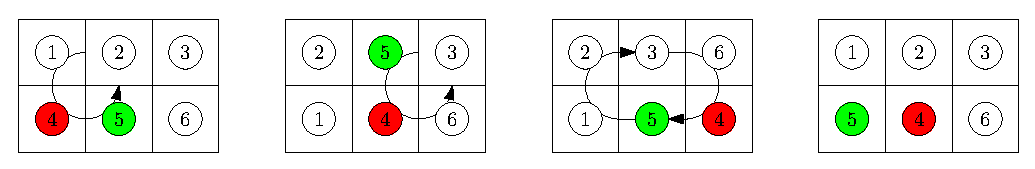
\includegraphics[width=0.8\linewidth]{ipe/swap_ex.eps}
	\caption{
		Swapping robots the red and green robots in three steps using a fixed amount of space.
	}\label{fig:swap3}
\end{figure}

\cite{algorithmica/MarbergG88} introduced an efficient algorithm called \emph{Rotatesort} which can sort a discrete \(n_1 \times n_2\) grid of \emph{elements} in parallel in \(\mathcal{O}(n_1 + n_2)\) time.
Rotatesort is not built with robots in mind, and uses only swap operations: swapping the positions of two adjacent elements.
We consider two swaps to be \emph{disjoint} when their four associated positions are distinct (i.e.~swaps \(4 \leftrightarrow 5\) and \(1 \leftrightarrow 2\) in \cref{fig:swap3} for example).
At any timestep, Rotatesort requires that we can execute any disjoint swap operations in parallel.

These operations obviously break the non-swapping constraint in \cref{req:no_swaps} of our robot motion planning problem. 
However, as seen in \cref{fig:swap3}, we can clearly simulate an atomic swap operation in \(\mathcal{O}(1)\) time for any single swap.
This can be executed in parallel for swaps in disjoint \(2 \times 3\) rectangles, and by repeatedly overlapping the rectangles in different patterns for \(\mathcal{O}(1)\) times we can simulate any single transformation step of Rotatesort in constant time.

As \(\mathcal{O}((n_1 + n_2) \cdot \mathcal{O}(1)) = \mathcal{O}(n_1 + n_2)\), this implies that for an \(n_1 \times n_2\) workspace there is an efficient algorithm that can always compute a schedule with \(\mathcal{O}(n_1 + n_2)\) makespan. 
This works for workspaces with densities of up to 100\%, i.e.~no free vertices available.

% As longer distances would ideally be traversed monotonously moving in the same direction, and not back and forth, continuously transforming \(n_1 \times n_2\) rectangles, \cite{siamcomp/DemaineFKMS19} comes up with the idea of combining Rotatesort with so-called \emph{subflows}. 

\subsection{Utilizing subflows to achieve constant stretch}

Building upon the previous findings, \cite{siamcomp/DemaineFKMS19} further details an algorithm for achieving a \emph{constant stretch factor} for arbitrary problem instances.

They make use of a technique that they call a \emph{subflow}, where robots going in the same direction get put in a queue, such that robots going in the same direction move efficiently without the need for simulated swap operations.

They first partition the workspace into large \(\mathcal O (d)\) tiles in a grid.
Any permutations within the tiles can then be executed in \(\mathcal O (d)\) steps, using the findings from \cref{alg:rotatesort}.

The tiles are by construction larger than the value \(d\), which means any robot has its target position within the eight tiles surrounding the tile that contains its starting position.
The many subflows cannot intersect each other though, i.e.~there cannot be two diagonal subflows perpendicular to each other in a \(2 \times 2\) square of tiles.
One can eliminate these intersecting subflows by first exchanging some robots between adjacent tiles in a preprocessing step, which can be executed in \(\mathcal{O}(d)\) time \cite{siamcomp/DemaineFKMS19}.

\cite{siamcomp/DemaineFKMS19} then show that \(\mathcal{O}(d)\) non-intersecting subflows can be used to move all robots to their target tiles, using \(\mathcal{O}(d)\) transformation steps.
With all robots in their target tiles, \(\mathcal{O}(d)\) steps are used to transform each tile into its target configuration using simulated Rotatesort.

On a very high level, the algorithms then works as follows:
\begin{enumerate}
	\item Compute a tiling of the workspace
	\item Preprocess between tiles to avoid intersecting subflows in \(\mathcal{O}(d)\) steps
	\item Move all robots to their respective target tiles using subflows in \(\mathcal{O}(d)\) time
	\item All robots are now in their target tiles. Transform all tiles to their target configurations in parallel in \(\mathcal{O}(d)\) steps
\end{enumerate}




% As a result, on a very high level, the following algorithm allows for a constant stretch schedule for any arbitrary workspaces with up to 100\% densities: 

The schedule for this can be computed in \(\mathcal{O}(dn_1 n_2)\) time \cite{siamcomp/DemaineFKMS19}, and it can be executed in \(\mathcal{O}(d)\) time.
\(\mathcal{O}(d)\) is equivalent to \(\mathcal O (L)\) (from \cref{def:stretch_factor}, see \cref{rem:d_and_L}), which implies a constant stretch factor, which also implies a constant approximation factor. 

